\chapter{Solution}
\label{solution}
\lhead{Chapitre 3 - Solution}
\section{Introduction}
Ce chapitre vise, à l'aide d'un exemple concret d'utilisation,  à 
\begin{enumerate}
\item expliquer les différents concepts de l'application. La section relative aux contraintes répondra aux deux questions suivantes;
	\begin{itemize}
		\item Comment les contraintes sont vérifiées et représentées?
		\item Comment les données sont importés, modifiées et représentées?
	\end{itemize}
\item décrire l'architecture de l'application,
\item détailler son implémentation.
\end{enumerate}

Un des principaux objectifs de ce mémoire étant d'offrir une solution maintenable et évolutive, l'application est divisée en trois parties distinctes, indépendantes entre elles. 

Ces trois parties sont les suivantes:
\begin{itemize}
\item l'import et la mise à jour des curricula, des cours et des différentes contraintes; 
\item la création du programme par l'étudiant, via l'interface utilisateur;
\item la vérification des différentes contraintes induites par le programme créé précédemment par l'étudiant.
\end{itemize}

\subsection{Exemple d'utilisation}

Tout au long de ce chapitre, l'exemple suivant va être utilisé pour illustrer le fonctionnement de l'application. Il s'agit un catalogue de cours fictif proposant deux programmes de cours.

\begin{figure}[H]
\centering
\caption{Exemple fictif de catalogue de cours}
% \label{running_example}
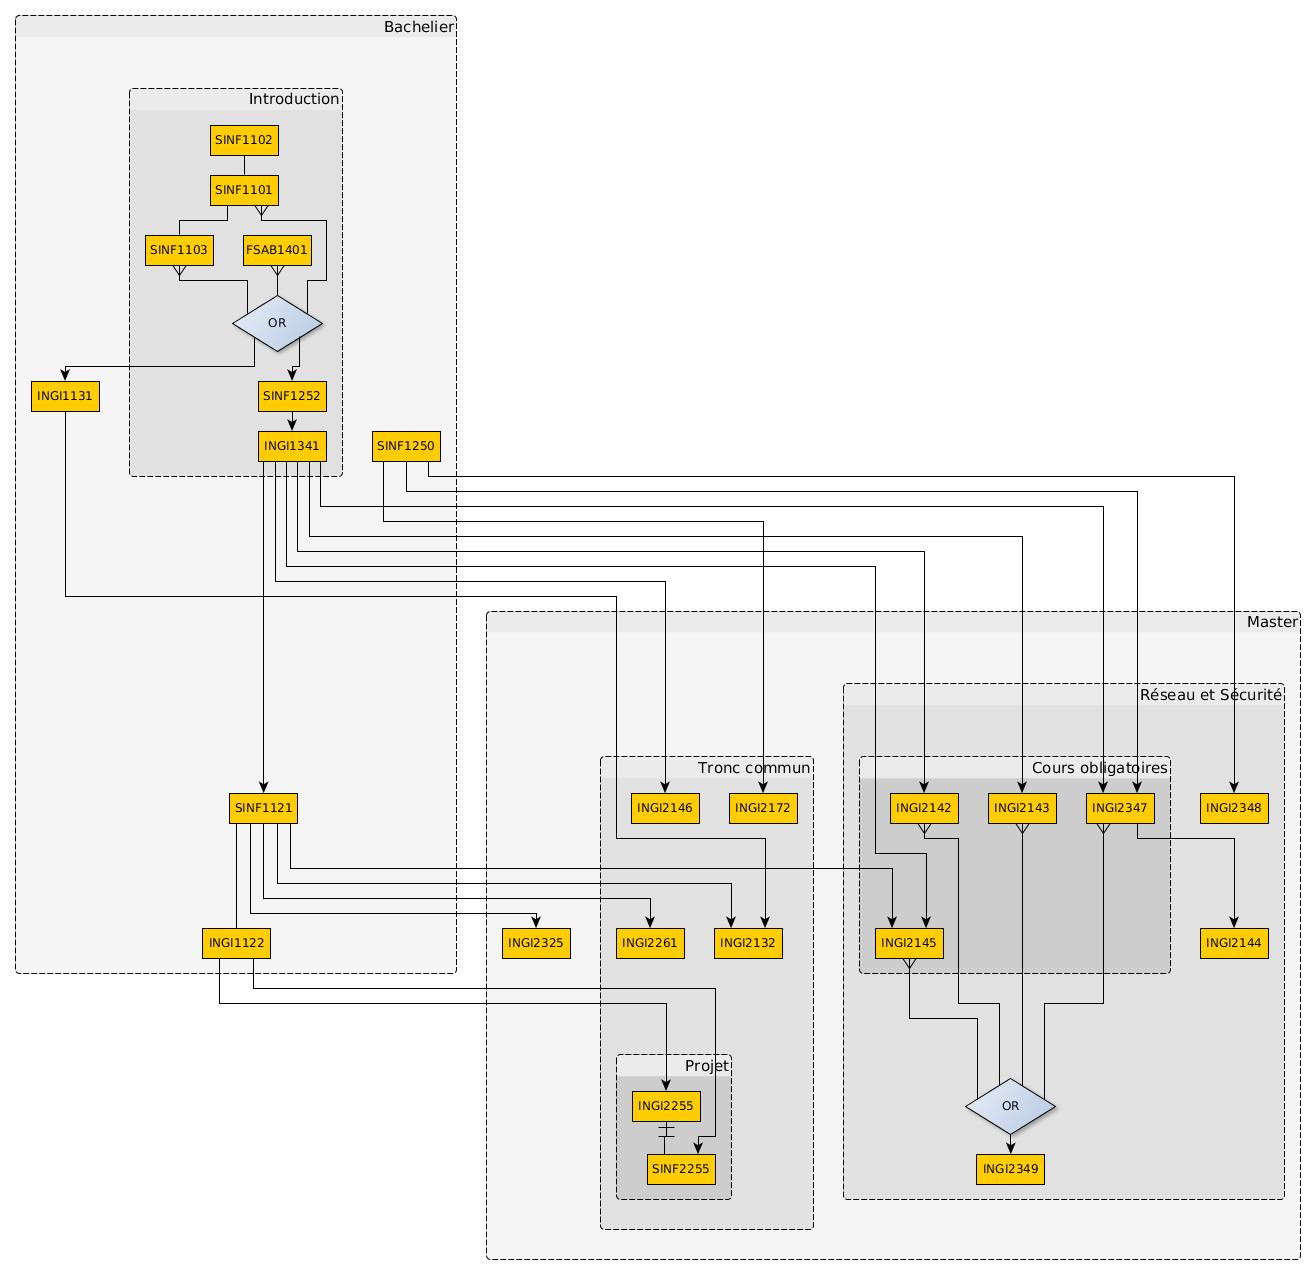
\includegraphics[width=\textwidth]{running_example}
\end{figure}

Ce catalogue est composé de deux programmes de cours.

Un programme de \textbf{Bachelier} composé d'un module obligatoire (Introduction)

Un programme de \textbf{Master} composé d'un module optionnel (L'option réseaux et sécurité) et d'un module obligatoire (Le tronc commun). Certains des cours de ce programmes ont des dépendances dans le programme précédent.  

 

\subsection{Processus désiré (à bouger vers le chapitre 1 ou 2)}
L'idée est d'améliorer le processus actuel, tel qu'illustré dans l'image ~\ref{fig:initial_process} du chapitre~\ref{introduction} vers le processus suivant \ref{fig:actual_process}

\begin{figure}[H]
\centering
\caption{Processus de création de programme avec l'application}
\label{fig:actual_process}
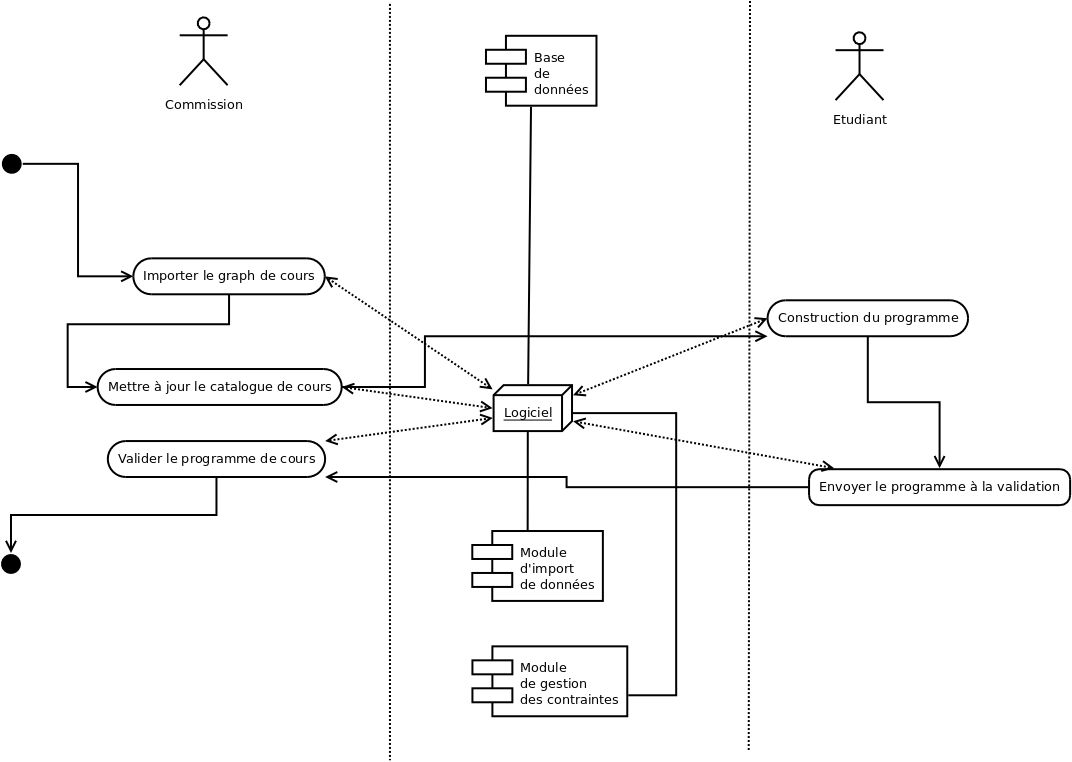
\includegraphics[width=0.8\textwidth]{actual_process}
\end{figure}

L'application est la nouvelle plateforme qui tient le rôle d'intermédiaire entre la commission et les étudiants. Elle est représentée par l'entité \textit{Logiciel} sur le diagramme \ref{fig:actual_process}. Il y a trois modules attachés à cette entité.

\textbf{Le module d'import de donnée} - Il permet à la commission d'enregistrer les données liées aux curricula  à l'aide de plusieurs supports (qui seront expliqués en détail plus loin dans le chapitre). Ce module permet tout d'abord d'ajouter considérablement plus d'informations dans le support confié à l'étudiant pour qu'il construise sont programme. Ensuite, il permet à la commission de mettre à jour facilement ces informations. 
 
\textbf{Le module de gestion des contraintes} - Il vérifie la validité des programmes créés par les étudiants.L'intérêt de ce module est de réduire considérablement  le temps que doit consacrer la commission à la correction des programmes d'étudiants. Premièrement, il empêche les étudiants d'envoyer leur programme à la validation s'il n'est pas correcte. il fourni aux étudiants un compte-rendu en temps réel de l'état de leurs programmes, en leur pointant les parties qui ne respecte pas les contraintes, quelles contraintes ne sont pas respectées et ce qu'il faut changer dans leur programme pour y remédier.

\textbf{La base données} - Elle stocke les informations liés aux curricula enregistrés précédemment par la commission, mais aussi les programmes des étudiants. La commission pourra avoir accès aux anciens programmes de cours, à tout les programmes des étudiants. Ces derniers quant à eux, pourront accéder aux différents programmes qu'ils ont déjà suivit et avoir une vision claire de ce qu'il leur reste à valider pour voir leur diplôme.

\subsection{Feuille de route}
Tout d'abord, il sera question des choix faits au niveau des technologies utilisées pour développer par l'application. Ensuite, l'architecture de l'application sera expliquée en détail. Après, les différents concepts de la solution seront présentés en détails. La dernière section sera consacrée à l'implémentation de la solution
\clearpage

\section{Technologies utilisées}
\subsection{Introduction}
Le but poursuivit par cette section est de présenter les différents choix faits aux niveaux des technologies utilisées par l'application. Ces choix sont de deux types. Premièrement, les technologies utilisées pour construire l'application seront présentées, comme le framework ou la base de données qui est utilisée. Les technologies externes à l'application qui sont utilisées pour construire les différents curricula ou mettre à jour leur informations seront présentées par la suite.

On parle de technologie interne pour représenter celles qui sont utilisées pour développer les fonctionnalités de application. Les technologies externes sont quant à elles des applications déjà existantes qu'il faut utiliser \textbf{en dehors} de l'application et pour lesquelles il ne faut pas écrire de lignes de codes.
\subsection{Ruby on Rails}
\subsubsection{Introduction}
Cette section a pour but de présenter la technologie principale utilisée pour développer l'application. Le but n'est pas de parcourir en détails le fonctionnement de rails, mais bien d'en présenter les concepts clés. En effet, il me semble important d'en comprendre les grande lignes, car son architecture, aussi bien que ses principes ont influencé la structure de la solution.
\subsubsection{Le choix d'un framework}
A première vue, l'utilisation d'un framework n'est pas absolument nécessaire. Cependant, un framework apporte toute une collection d'outils qui aident à développer mieux et plus rapidement.

\textbf{Mieux} car il permet de développer une application qui est structurée, ce qui rend le code plus maintenable et évolutif.

\textbf{Plus rapide} car il permet de gagner du temps en réutilisant des modules génériques afin de se concentrer sur d'autres domaines. Avec un framework, on assemble des briques plutôt que de réinventer la roue. 

Enfin, le dernier atout d'un framework se situe au niveau de l'intégration de nouveaux développeurs sur le projet. Dans le cadre de ce mémoire, il est clair que de nouvelles fonctionnalités devront être ajoutées dans le futur. De plus, les fonctionnalités existantes devront peut être modifiées ou améliorées. Il sera plus facile pour cette personne de se plonger dans du code qui n'est pas le sien, s'il a une structure propre aux standart web d'aujourd'hui.

\textbf{Il est donc fortement conseillé d'utiliser un framework web pour créer ce genre d'application.} 

Il en existe une multitude aujourd'hui. Il y a tout d'abord les frameworks PHP comme CakePHP, DRUPAL ou Symfony (pour ne citer que les plus connus). Vient ensuite Ruby on Rails, un framework en ruby et Django, un framework en Python.  
\subsubsection{Le choix de Ruby on Rails}
L'intérêt réside dans le niveau de productivité et de maintenabilité accru que l'on obtient en travaillant avec le framework. Les design pattern sous-jacents, et la philosophie de Rails permettent de concentrer son travail sur les fonctionnalités de l'application plutôt que de passer son temps à écrire du code répétitif ou remplir des fichiers de configuration. 

De plus, il existe une multitude de librairies tierces appelées \textit{ruby-gem} qui réduisent encore le nombre de lignes de codes à produire, en apportant des fonctionnalités à l'application. Le meilleur exemple est \textbf{devise}, une librairie qui permet d'ajouter la gestion de l'utilisateur(création, connexion, récupération de mot de passe, envois de mails, etc ..) en quelques lignes en plus de gérer les sessions et les accès aux différentes actions et vues. 

Rails pousse aux bonnes pratiques, c'est d'ailleurs cette philosophie qui m'a incité à développer la plupart des fonctionnalités, comme vous le verrez plus tard, dans des librairies externes à l'application.


En outre, Rails dispose d'une communauté très active et passionnée, qui teste, documente et améliore les fonctionnalités du framework. 
\subsubsection{Limites}
Les limites du framework sont les suivantes
\begin{itemize}
\item Lorsque l'on débute, on est souvent tenté de charger les modèles en voulant suivre la philosophie \textit{tiny view - skinny controller - fat model}\footnote{Bonne pratique qui consiste à délaisser toute la logique aux modèles} et l'on oublie souvent qu'il est possible de déléguer la plupart des fonctionnalités à des librairies externes, qui sont plus faciles à développer - car crées en pure \textit{ruby} - et plus facile à tester - car indépendantes de rails \cite{fat_models}.

\item (...)
\end{itemize}

\subsubsection{Conclusion}
Le choix s'est naturellement porté Ruby on Rails. C'est un framework open-source, utilisé pour développer des applications web. Le développement se fait à travers le langage de programmation multi-paradigmes (Programmation fonctionnelle, orientée object, ...) \textbf{ruby}. Il se base sur des puissants design patterns et principes qui vont être présentés en quelques lignes ci-dessous.

\subsubsection{DRY - Don't repeat yourself}
Comme son nom l'indique, ce premier principe pousse à la réutilisation du code existant le plus souvent que possible, plutôt que d'avoir des bout de codes similaire un peu partout dans l'application. L'idée de tendre vers une structure \textit{Api}, où tout ce qui n'est pas nécessaire aux classes et méthodes externes est caché en interne. Le principal avantage se situe au niveau de la \textbf{maintenabilité}. On évite ainsi de devoir partir à la recherche des différents bouts de code dupliqués lorsque l'on veut modifier le comportement d'une méthode, d'une classe, ou même d'un module.

\subsubsection{CoC - Convention over Configuration}
L'idée est de réduire au minimum les décisions à prendre avant de commencer à développer. Une convention importante en \textit{Ruby on rails} se situe au niveau des noms des classes pour lesquelles il existe une table correspondante en base de données. Pour un modèle \textit{Course} par exemple, la convention est d'avoir une table nommée \textit{courses} en base de données. Cela permet d'éviter d'avoir à écrire du code supplémentaire pour spécifier à l'application quelle table correspond à quel objet. 

Cela permet au développeur de se concentrer sur les parties non conventionnelles de l'application, comme l'architecture, plutôt que de perdre son temps à configurer les objets. L'avantage ici se situe plus au niveau de la \textbf{productivité}.
\subsubsection{MVC - Model-Vue-Controlleur}

Le framework s'appuie sur le pattern \textbf{MVC}. Destiné aux applications dites \textit{interactives}, il divise l'application en trois parties; le modèle, les vues et le contrôleur. Notez que \textit{Ruby on Rails} ne respecte pas totalement MVC dans sa conception initiale. Cela se justifie par le fait que ce pattern n'est pas destiné à la base aux applications web, notamment car la vue est ici une page web. Le modèle ne peut donc pas lui envoyer tous les changements qui surviennent au niveau des données. C'est la vue, qui doit expressément faire les requêtes pour ces données, à travers le contrôleur.

MVC à la sauce Rails se présente comme suit. Nous avons

\begin{itemize}
\item Le \textbf{modèle}, lié à une base de données, qui contient les données et l'état de l'application. Il contient aussi toute la \textit{business logic}, qui détermine comment l'information est créée, mise à jour, et affichée.
\item Les \textbf{vues} qui génèrent l'interface utilisateur et lui présente les données. Ce composant est passif, il ne traite aucune information. \textit{Vues} est au pluriel ici, car plusieurs vues peuvent avoir accès au même modèle. 
\item Le \textbf{contrôleur} qui reçoit les événements du monde extérieur, interagit avec le modèle et choisit la vue à afficher à l'utilisateur. Par exemple, lorsque l'utilisateur veut éditer un commentaire dans un blog, le contrôleur va rendre la vue relative à l'édition de l'objet correspondant. 
\end{itemize} 

\subsubsection{Active Record}
Ce pattern quant à lui stocke les données dans une base de données relationnelle. Il s'agit simplement de fournir une abstraction supplémentaire à la base de données et fournir des fonctions pour manipuler les données. Dans le cas de rails, il y a donc une couche ruby entre la base de données proprement dite et la logique dans notre modèle. Cela permet par exemple, d'être indépendant du système de base de données utilisée en dessous.  Par exemple, \textit{postgresql} est le système de gestion de base de données utilisé pour le moment. Si pour une raison X ou Y, il devient nécessaire de passer à \textit{sqlite3}, il suffit de changer le fichier de configuration \textit{config/database.yml} de
\begin{lstlisting}
development:
  adapter: postgresql
  database: db/development
  pool: 5
  timeout: 5000
\end{lstlisting}
vers
\begin{lstlisting}
development:
  adapter: sqlite3
  database: db/development
  pool: 5
  timeout: 5000
\end{lstlisting}

Et de recréer la base de données avec
\begin{lstlisting}
rake db:create:all
rake db:migrate
\end{lstlisting}

(source : \cite{rails_cast_migration_to_postgresql}

Tout cela est fait sans devoir changer la façon dont j'accède aux données dans les différents modèles.  

\subsection{Base de données - PostgreSQL}

Rails supporte plusieurs systèmes de gestion de base de données : (PostgreSQL, MySQL, SQLite). Le choix du système est cependant restreint à l'outil utilisé pour héberger l'application. En effet, il est nécessaire d'avoir une base de données PostgreSQL pour pouvoir héberger l'application sur la plateforme. 

\subsection{Éditeur de graphes - yEd}

Comme expliqué plus tard dans la section gestion des données, le choix s'est porté vers une importation en deux parties des données dans l'application. Pour ce faire, il est nécessaire de construire un graphe de cours pour représenter le catalogue contenant les différents programmes de cours proposés par la \textit{commission INFO}.

Plusieurs alternatives se sont présentées.

La première correspond à un logiciel intégré dans l'application, qui permet de construire explicitement un catalogue de cours sous forme de graphe, en proposant exclusivement de placer des objets cours, modules, ou programmes sur le graphe et en n'offrant que des arrêtes de type corequis ou prérequis. Cette application communiquerait directement avec les modèles et permettrait de générer directement les objets (cours, modules, ...) désirés. Cependant il n'existe pas d'applications réalisant ce genre de graphe pour le moment, et cela sort du cadre de ce mémoire

La deuxième alternative serait d'intégrer un outil générant des graphes plus standard dans l'application. YEd offre une solution très chère à ce sujet. Il y a aussi une librairie en Javascript assez souple (d3js ). Ces solutions implique quoiqu'il arrive de devoir parser les données par ces outils.

La troisième et dernière alternative serait d'utiliser un logiciel externe à l'application pour générer ces graphes. Ce logiciel doit être entre autre multi-plateformes (Mac os x, Linux \& Windows) et capable d'exporter dans un format relativement facile à parser. La liste de ce genre de logiciel est assez longue (Dia, Yed, OmniGraffle, Graphiz)
\begin{itemize}
  \item Dia - C'est un logiciel assez léger qui est capable d'exporter en Xml, un format standard pour représenter des données. Il devient cependant très ennuyeux à utiliser lorsque l'on manipule des graphes de taille importante.
  \item OmniGraffle - Ce logiciel n'est disponible que sur Mac Os X malheureusement.
  \item Yed - Ce logiciel est assez complet. Il est cross-plateforme et à l'avantage de contenir des algorithmes qui permettent de restructurer automatiquement les graphes. Il permet aussi d'exporter en deux formats de types xml (Graphml \& XGml)
  \item (...)
\end{itemize}

Étant donné la contrainte de temps imposé par le cadre du mémoire, le choix c'est porté vers un logiciel déjà existant. Il a été préférable de choisir une solution externe pour éviter de surcharger l'application avec de lourds modules graphiques. De plus, intégrer ce genre de logiciels dans l'application ne changeait rien au fait qu'il fallait parser le fichier exporté par l'outil pour importer les données dans l'application.

YEd a été choisi pour toutes ces raisons. 
\subsection{Xml}

\subsection{Excel}
\clearpage
\section{Architecture}
% Parler architecture contrainte, pourquoi un object contrainte et un object constraintSet
\subsection{Modèle de données}

\subsubsection{Architecture globale}

\begin{figure}[H]
\caption{Architecture globale}
\centering
\label{fig:complete_arch}
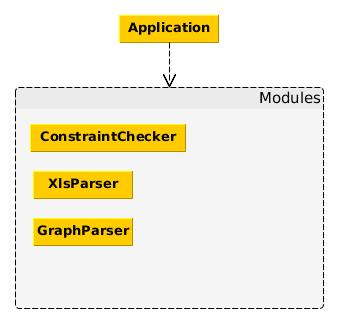
\includegraphics[width=\textwidth]{complete_arch}
\end{figure}

Ce modèle représente l'architecture de l'application et de l'ensemble de ses modules. L'objet application représente la partie \textit{Rails} de l'application. Cette partie comporte essentiellement les différents modèles, leurs vues et leurs contrôleurs. L'application utilise trois modules développés indépendamment.
\begin{enumerate}
  \item \textbf{GraphParser} - le module s'occupant de parser les fichier .Graphml générer par yEd, 
  \item \textbf{ConstraintCheker} - le module s'occupant de vérifier les contraintes des programmes d'étudiants
  \item \textbf{XlsParser} - le module occupant d'écrire et de lire dans des fichier excels. 
\end{enumerate}

L'architecture de chacun de ces modules, en plus de celle de l'application sera expliqué dans les sous-sections qui suivent.

Les conventions utilisées pour réaliser chacun des modèles sont les suivantes; 

\begin{figure}[H]
\centering
\caption{Généralisation}
\label{fig:generalization}
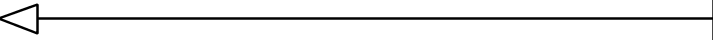
\includegraphics[scale=1]{generalization}
\end{figure}

\begin{figure}[H]
\centering
\caption{Dépendance}
\label{fig:dependancy}
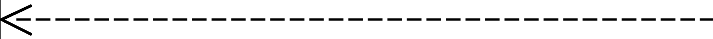
\includegraphics[scale=1]{dependancy}
\end{figure}

\begin{figure}[H]
\centering
\caption{Association ``has many''}
\label{fig:has_many}
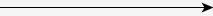
\includegraphics[scale=1]{has_many}
\end{figure}

\begin{figure}[H]
\centering
\caption{Association ``many to many''}
\label{fig:many_to_many}
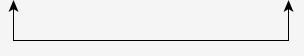
\includegraphics[scale=1]{many_to_many}
\end{figure}

\begin{figure}[H]
\centering
\caption{Représentationd d'un objet. En haut; les attributs, en bas; les méthodes.}
\label{fig:class_example}
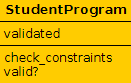
\includegraphics[scale=1]{class_example}
\end{figure}



\subsubsection{Application Rails}
\label{arch}
\begin{figure}[H]
\centering
\caption{Architecture de l'application}
\label{fig:app_arch}
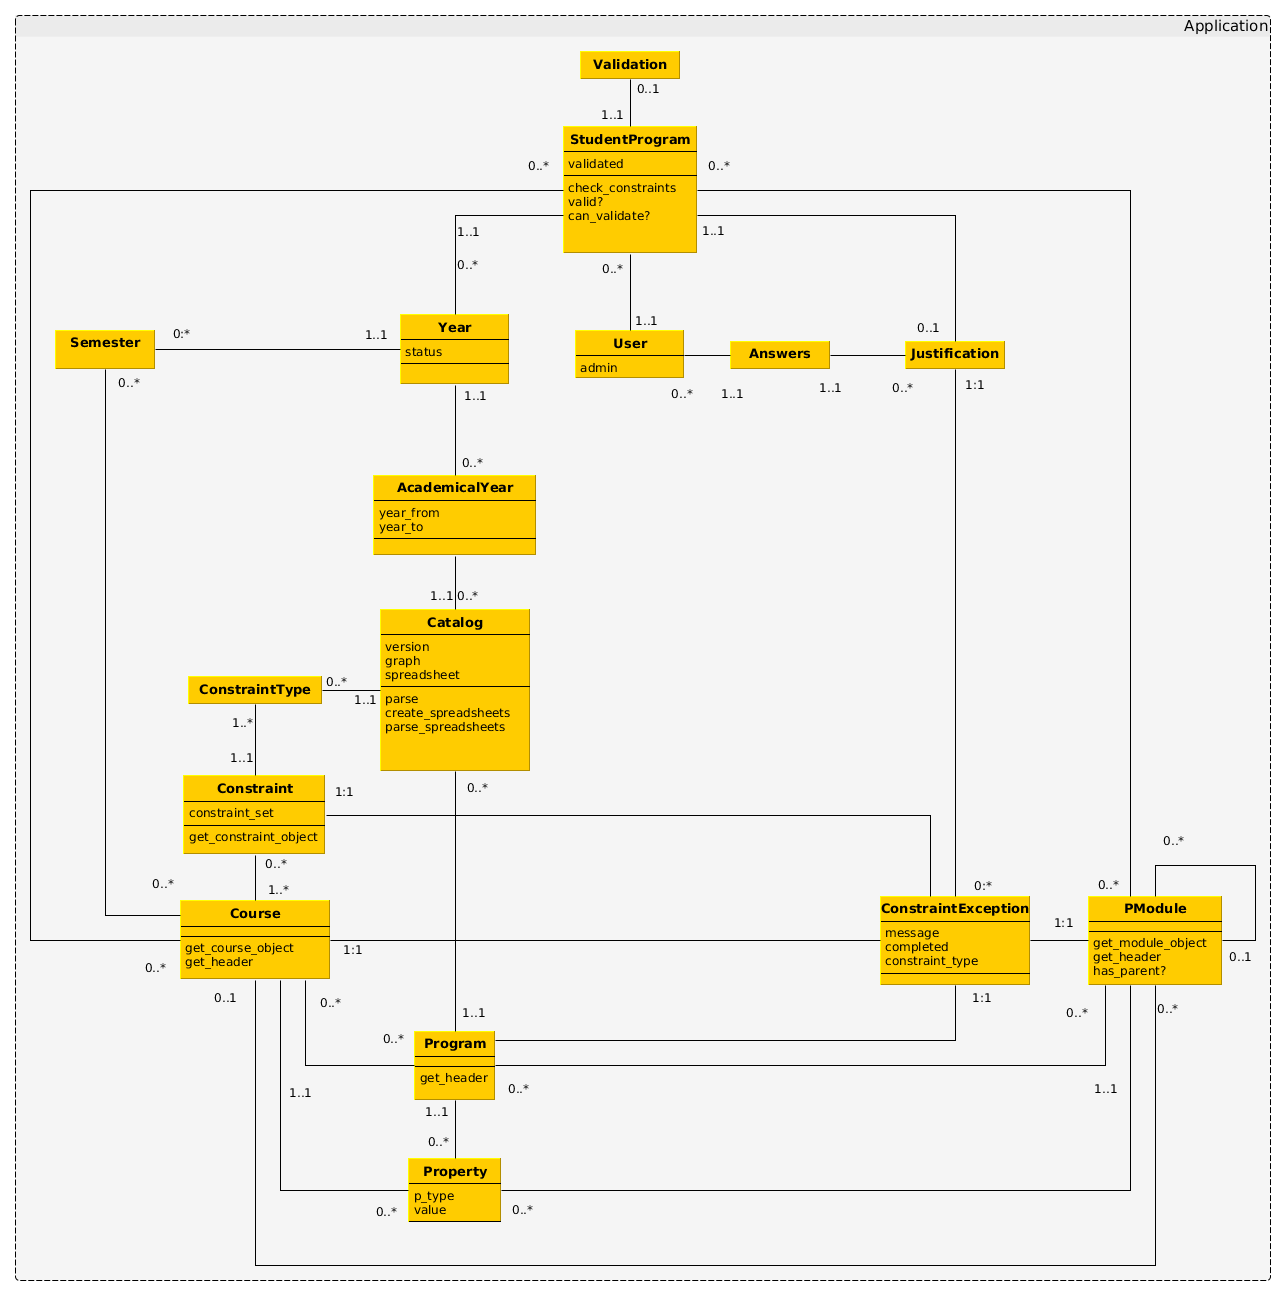
\includegraphics[angle=90, height=\textheight, width=\textwidth]{app_arch}
\end{figure}

\textbf{Student - Admin} - Ces objets représentent les deux acteurs de l'application, à savoir la \textit{Commission INFO} (Admin) et les étudiants (Student).

\textbf{Property} - Un objet \textit{Property} est composé d'un type et d'une valeur. Chacun des objets \textit{Program}, \textit{PModule} et \textit{Course} peut en avoir 0 ou plusieurs. Par exemple, pour représenter le sigle d'un cours, une propriété de type \textit{SIGLE} et de valeur \textit{SINF1101} sera ajoutée au cours correspondant. Il a été choisi d'opter pour cette solution, plutôt que d'ajouter des champs arbitraire (Sigle, crédits, ...) à chacun des objets car on ne sait pas à l'avance quelles seront leur propriété. En effet, elle sont déterminées par les informations mises dans le fichier excel qui est importé régulièrement dans l'application. 

\textbf{PModule} - C'est un ensemble de cours. Un \textit{PModule} peut avoir plusieurs \textit{PModule}. Ce comportement est justifié par le fait qu'un module de cours peut comporté un sous module qui comporte une série de cours obligatoires (L'option réseau et l'ensemble de ses cours obligatoires par exemple).

\textbf{Program} - Il représente un programme de cours. (Le programme de master par exemple) C'est un ensemble de cours et de modules divers. On peut créer des programmes via l'outil de graphes yEd, mais il est possible dans l'application de créer des Programmes \textit{à la carte} en choisissant les modules et cours qui le compose. C'est pourquoi il y a une relation \textit{many to many} entre \textit{PModule} et \textit{Program} et une autre entre \textit{Program} et \textit{Course}. En effet, chaque Programme peut avoir un ou plusieurs cours, et chaque cours peut appartenir à un ou plusieurs programmes (Le même comportement est observé pour les modules). Il n'est donc pas possible de représenter cette relation avec une relation \textit{has many} classique, qui implique d'avoir l'identifiant d'un des deux objets dans l'autre. \cite{active_record}. 
\textbf{Catalog} - Un catalogue est composé de plusieurs \textit{Program}, \textit{PModule} et \textit{Course}.

\textbf{StudentProgram} - C'est le programme que se crée l'étudiant lorsqu'il utilise l'application. Un \textit{StudentProgram} est une instanciation d'un des \textit{Program} disponible dans le \textit{Catalog} utilisé (d'où la relation \textit{many to many}). De plus, un étudiant doit choisir les modules qu'il va suivre. Ce comportement est expliqué par la relation \textit{many to many} entre les deux modèles. Pour configurer son programme année par année, l'étudiant va se créer une année (\textit{Year})

\textbf{Year} - Une année est composé de deux semestres. Un semestre est représenté par l'objet \textit{Semester}. Le choix de chacun des cours du semestre est représenté par l'association \textit{many to many} qui existe entre les deux objets. Pour représenter le premier et le second semestre, un modèle \textit{FirstSemester} et un modèle \textit{SecondSemester} ont été créés, tout deux étendant le modèle \textit{Semester} en utilisant la \textit{Single Table Inheritance} de \textit{Rails} \cite{STI}. Notez que la relation entre ces deux types de \textit{Semester} et leur \textit{StudentProgram} est une \textit{has one} (la cardinalité est donc (1, 1) ici)

\textbf{Header} - Chacun des modèles \textit{Course}, \textit{Pmodule} et \textit{Program} contient une méthode get\_header qui renvoie une suggestion de propriétés utilisées à titre indicatif avec le module \textit{XlsParser} (voir \ref{xls_parser}) pour créer les formulaires excel. Nous avons le header suivant : \{"SIGLE", "CREDITS", "SEMESTRE", "OBLIGATOIRE"\} pour le modèle \textit{Course} par exemple.  





\subsubsection{Architecture du vérificateur de contraintes}
\label{constraint_checker}
\begin{figure}[H]
\centering
\caption{Vérificateur de contraintes}
\label{fig:constraint_checker_arch}
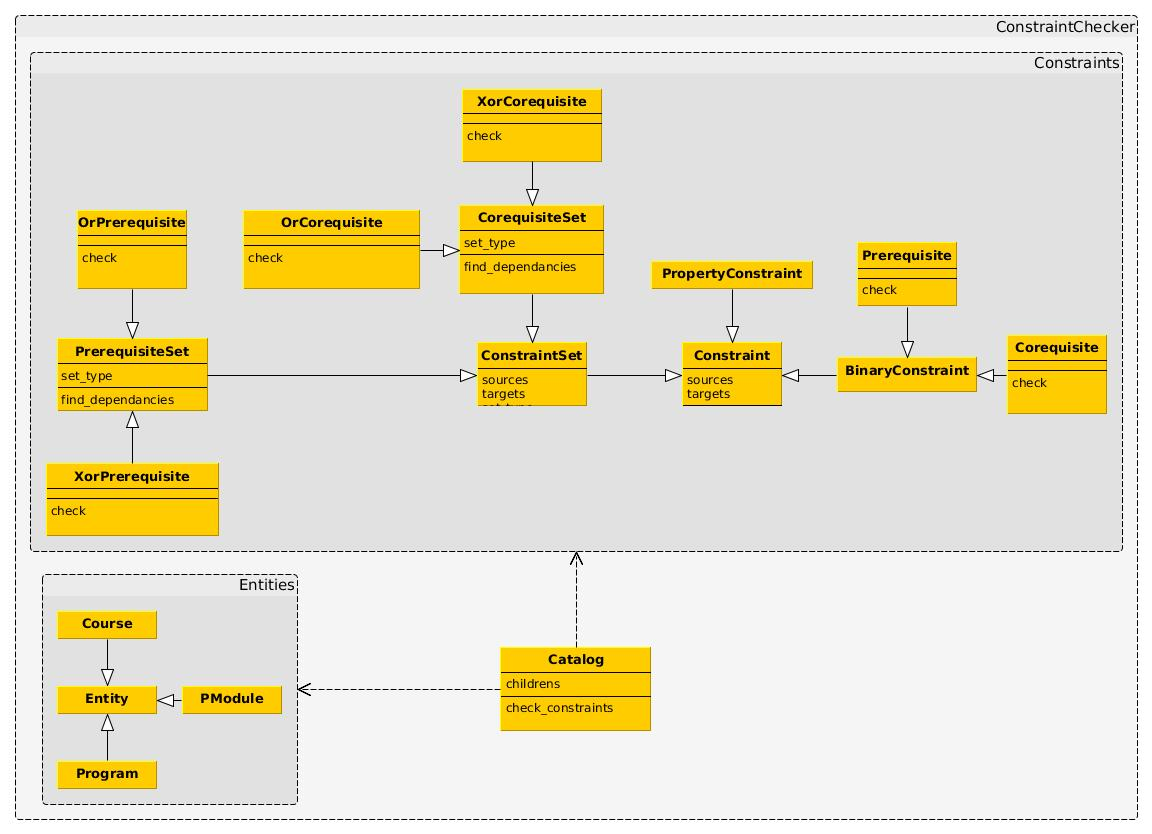
\includegraphics[width=\textwidth]{constraint_checker_arch}
\end{figure}

L'architecture de ce module est composé en deux parties;
\begin{enumerate}
  \item Les différents types de contraintes (Contraintes binaires, ensemble de contraintes ...)
  \item Les différents types d'entités (Cours, modules, ...)
\end{enumerate}

Le lien avec l'application se situe au niveau de la classe \textit{Catalog}. En effet, chacune des différentes entrées des tables concernées (courses, p\_modules, constraints) sont traduites en un objet entité.

L'idée ici est d'utiliser au plus l'héritage pour éviter d'avoir des duplications de code dans les classes. Par exemple, un objet \textit{Course} peut avoir beaucoup de contraintes mais chacune d’entre elles peut être de n'importe quel type. Cet objet n'a pas besoin de savoir le type de ses contraintes. Tout ce qu'il sait, c'est qu'il doit appeler leur méthode \textit{check} pour tester si les contraintes sont vérifiées. 


\subsubsection{Parser de graphes}

\begin{figure}[H]
\centering
\caption{Architecture du parser de graphe}
\label{fig:graph_parser_arch}
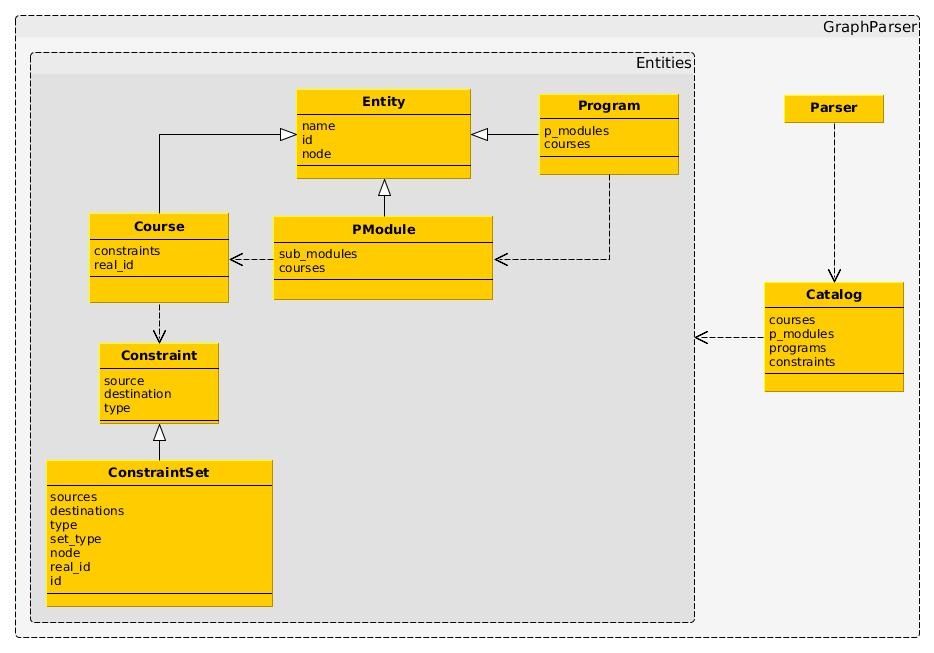
\includegraphics[width=\textwidth]{graph_parser_arch}
\end{figure}

Tout comme dans le vérificateur de contraintes \ref{constraint_checker}, le parser travail avec des objets \textit{entités} à la différence que c'est lui qui les fournit à l'application (et pas l'inverse)

De nouveau, l'héritage tient une page prépondérante ici, pour diminuer le couplage, augmenter la cohésion  et éviter autant que possible la duplication de code \cite{cohesion_couplage}. 

\subsubsection{Parser de fichiers excel}
\label{xls_parser}
\begin{figure}[H]
\centering
\caption{Architecture du parser de fichiers excel}
\label{xls_parser_arch}
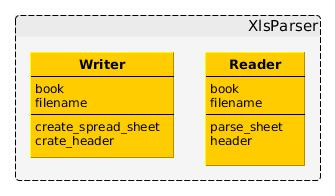
\includegraphics[scale=1]{xls_parser_arch}
\end{figure}

Ce module est relativement simple; il est composé de deux classe, un \textit{Writer} qui prend en input un tableau de donnée et un \textit{Reader} dont l'output est aussi un tableau de donnée.


\clearpage
\section{Conception}
\subsection{Contraintes}
Les contraintes comme présentées dans les sous-sections qui suivent, sont de plusieurs type. Cette catégorisation est nécessaire pour plusieurs raisons. 

Premièrement, elles ne sont pas représentées de la même façon de la même façon. En effet, certaines sont représentées par un object en base de données (Les dépendances entre les cours). D'autres, n'ont pas de représentation à proprement dite, dans le sens où elles n'ont pas un object appelé contrainte pour les représenter, car elles portent sur des champs de certains objets. 

Deuxièmement, leur données ne sont pas importées de la même façon. 

Enfin, elle ne sont pas vérifiées de la même manière. Ces différences, comme vous le verrez dans la partie Implémentation on justifié le choix d'implémenter cette gestion des contraintes dans un module externe à \textit{Ruby On Rails}, pour permettre s'abstraire ces contraintes en un et unique object Contrainte, qui lui même connaît
\begin{itemize}
\item ses données. Par exemple, une contrainte spécifiant le minimum de crédits pour un module connaît l'objet sur lequel cette contrainte s'applique et la valeur de celle ci.
\item la logique intrinsèque de cette contrainte. Toujours pour ce minimum de crédits requis, la méthode de vérification propre à ce type de contrainte sait qu'il faut calculer la somme des crédits des cours de l'objet Module sur lequel elle s'applique. 
\end{itemize}    
\subsubsection{Dépendances}
TODO AJOUTER IMAGES
Ces contraintes portent sur les cours. 
Elle sont de deux types:
\begin{enumerate}
\item Les prérequis : exprimant les cours qu'il est nécessaire d'avoir suivit pour pouvoir suivre le cours
\item Les corequis : exprimant les cours qu'il est nécessaire de suivre durant la même année académique que le cours sur lequel la contrainte s'applique. 
\end{enumerate}

De plus, il existe aussi des disjonctions de contraintes, exprimant qu'il faut
\begin{itemize}
\item avoir suivit un des cours pour pouvoir suivre le cours en question (Conjonction de prérequis)
\item suivre un des cours de la liste durant la même année académique que le cours en question (Conjonction de corequis)
\end{itemize}

Ces contraintes sont importées dans l'application via l'éditeur de graph yEd. Elle sont représentées par les arrêtes entre les différents nœuds dans le graphe. 
\subsubsection{Contraintes sur les propriétés}
TODO : AJOUTER IMAGES
Ces contraintes portent sur les programmes, les modules, les sous-modules et les cours. Elle représentent n'importe qu'elle type de contrainte qui pourrait exister sur les champs \textit{Property} de ces objets. Un exemple serait les 180 crédits nécessaires à la validation d'un programme de \textbf{BAC}

Les données relatives à ces contraintes n'ont pas de représentation en tant que telles dans la base de données, c'est à dire qu'il n'y a pas d'objet \textit{PropertyConstraint} qui les représente. La principale raison qui justifie ce choix est la suivante:

Ces contraintes portant sur les propriétés des objets, elles sont importées via le formulaire excel dans l'application. Or, il n'y a pas une contrainte par propriété, on ne peut donc pas créer une contrainte par propriété, cela n'aurait pas de sens. (On a par exemple, pour un cours, son sigle, son nom complet, le professeur, l'url du cours sur le portail de l'ucl, ses crédits, etc). 

On pourrait créer une nouvelle page par objet dans le formulaire excel, pour représenter seulement les contraintes de l'objet en question. Cependant, il faudrait ajouter beaucoup de logique dans les modèles pour exprimer que tel propriété est une contrainte. Tout dépendrait des données que l'ont met dans le formulaire. Si la personne qui utilise l'application est fatiguée et se trompe dans le nom de la page, ou du nom de l'objet, ou encore du nom de la contrainte, la création de celle-ci ne fonctionnera pas. Pire, elle pourrait ajouter des contraintes correctes dans la forme, mais qui s'appliquent à d'autres objets. Il est très difficile de vérifier ce genre d'erreurs. 

Ce genre de solution n'était pas du tout souple et source de beaucoup d'erreurs, il a été préférable de partir dans une autre direction. 
\begin{enumerate}
\item Laisser ces contraintes exprimées implicitement dans la base de données (= Pas d'objet \textit{PropertyConstraint}).
\item Délayer la logique de ces contrainte au module du même nom, en demandant au module de passés les informations nécéssaires à ces contraintes au module. 
\end{enumerate} 
\subsubsection{Contraintes temporelles}
TODO
\subsection{Gestion des Données}
\label{gestion_des_données}
\subsubsection{Introduction}
Cette section répond à la question de comment sont importées les données relatives aux programmes, leur cours, leurs informations et leur différentes contraintes. 

Les différentes informations contenue dans le catalogue de cours du département sont les suivantes. Nous avons
\begin{itemize}
\item Plusieurs programmes de cours (BAC SINF et INFO, MASTER SINF et INFO, Passerelle SINF et toute les options qu'elles contiennent)
\item Chacun de ces programmes contiennent des modules et des cours, avec des informations relatives aux cours et modules obligatoires.
\item Chacun de ces cours peut avoir des dépendances. (Voir section contrainte pour plus de détails)
\end{itemize}

Il faut donc trouver un moyen de télécharger ces informations dans l'application. La solution la plus naïve serait de fournir des formulaires pour chaque entité (Cours, modules, ...) permettant d'ajouter une à une toute les informations nécessaire. Si l'on veut modifier les informations d'une entité, \textit{"il suffirait"} de naviguer dans les différents menu et de sélectionner le menu d'édition correspondant. Cependant cette solution n'atteint pas l'objectif fixé dans la solution, à savoir fournir un support pour enregistrer efficacement (et donc en peu de temps) les informations relatives aux curricula. Ajouter une à une toute les dépendances de cours peut être très ennuyant. 

Une première amélioration que l'on peut ajouter à cette solution, est d'utiliser des formulaires excel pour ajouter ces informations. En créant une page par entité comme présenté sur l'image~\ref{fig:excel_example}, on pourrait ajouter toute les informations liés au modules, aux cours plus efficacement, l'import de fichier excel étant une chose assez aisée. 
\begin{figure}[H]
\centering
\caption{Feuille Excel pour importer les données relatives aux modules}
\label{fig:excel_example}
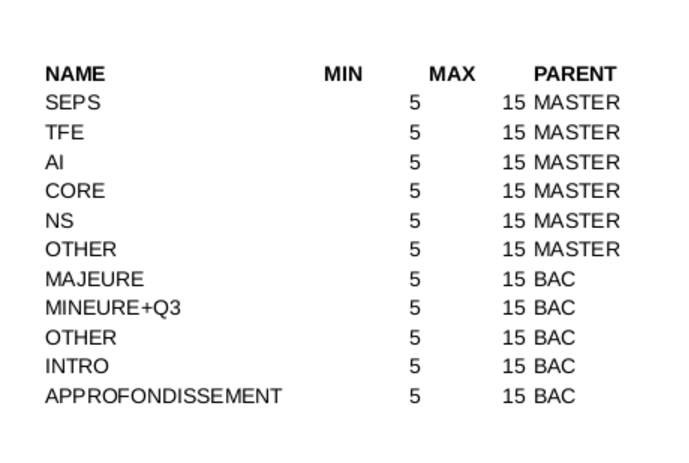
\includegraphics[width=0.8\textwidth]{excel_example}
\end{figure} 

Bien que cela permette d'ajouter des informations de façon plus efficaces, il subsiste plusieurs problèmes
\begin{itemize}
\item C'est toujours aussi éprouvant d'ajouter les dépendances. Il toujours les ajouter une par une, bien que cela soit sur une seule page.
\item On ne peut pas donner au formulaire (et le programme qui l'importe) le pouvoir de créer les entités car:
\begin{itemize}
	\item En cas de faute de frappe, il faudra de nouveau naviguer dans l'application pour supprimer les erreurs.
	\item Il est très difficile et peu efficace de gérer les inclusions des cours(L'appartenance d'une entité à une autre, un cours à un module par example). Cela implique des recherches sur le nom des entités. De nouveau, en cas de faute de frappe, il faudra aller corriger les erreurs dans l'application
\end{itemize}
\end{itemize}

Le catalogue de cours étant un graphe (Dont les nœuds sont des entités et les dépendances des arrêtes), une autre solution serait d'utiliser un logiciel qui permet d'en dessiner. Un graphe étant visuellement plus parlant  qu'un tableur, le nombre d'erreurs serait donc moindre. 

Le principal problème de cette solution réside dans les informations que l'on peut mettre dans ce graphe. Certes, on pourrait \textit{bricoler} avec le logiciel pour ajouter des méta-données aux objets que l'on dessine, mais cela pourrait de nouveaux devenir très embêtant à utiliser et surtout relativement compliqué à importer. 
  
La solution utilisée dans l'application est un compromis entre la solution \textit{"graphe"} et celle \textit{"excel"}. La gestion des données est subdivisées en deux processus:
\begin{itemize}
\item L'import de la structure du catalogue via un logiciel qui permet de dessiner des graphes
\item L'ajout d'informations supplémentaires (Nom, crédits, ...) via un import de formulaire excel
\end{itemize}
\subsubsection{Pourquoi avoir subdiviser l'import des données en deux parties distinctes?}

Pour rendre les choses plus aisées au personnel qui va encoder le programme, nous avons décidé d'utiliser yEd, un outil relativement haut niveau qui permet de générer des graphes. En peu de temps, il est possible de construire l'ensemble du programme de cours à l'aide de cet éditeur disponible sur Windows, Mac Os et Linux tout en sortant un diagramme clair et concis.


\textbf{Pourquoi}? Car le programme de cours est un graphe, dont chaque nœud correspond à un cours et chaque \textit{edge}, à une dépendance. 

La solution idéale serait d'avoir un logiciel qui, en plus d'être intégré à l'application serait totalement adapté à notre besoin, à savoir \textbf{dessiner un graphe de cours}. Cela serait un dessinateur de programme de cours à part entière, proposant des nœuds intitulés cours, des arrêtes pour exprimer les contraintes, une façon de regrouper ces nœuds en module, en plus d'une autre pour y ajouter des informations relatives aux crédits, au contraintes des modules, etc. Cependant, cela dépasse malheureusement le cadre de mon mémoire. Libre à un étudiant, féru de développement web, de s'y attaquer dans les années à venir.

\subsubsection{Limites de la démarche}
Pour revenir à la façon dont nous importons les données, la principale limite d'un outil de la sorte est que nous sommes limités dans l'information que nous pouvons mettre dans ce graphe. Certes, il serait possible de sélectionner les différents nœuds et modules un à un et d'y ajouter l'information nécessaire, mais cette solution n'est pas efficace. Ils existe des solutions plus efficaces pour gérer des données à grande échelle : Excel.

La seconde limite, est qu'il faut se mettre d'accord sur l'utilisation de ce programme tiers afin de savoir \textit{quoi} parser. Tout cela sera détaillé dans un manuel disponible dans les annexes

L'import des données se fait donc en deux temps. Le graphe, qui contient les informations sur la structure du catalogue de cours (Nom des différentes entités et des dépendances), est d'abord parsé par l'application pour en extraire les informations. En suite, les informations plus spécifiques du catalogue de cours (les propriétés diverses des entités; nom détaillé, url, date, informations sur les crédits) doivent être fournies via un formulaire Excel qui, à sont, tour doit être télécharger vers l'application.

\subsubsection{Construction et Import de la structure du catalogue}
L'idée est de construire le graphe de cours en utilisant une application externe. Les exigences pour ce logiciel sont les suivantes:
\begin{itemize}
\item  Avec ce logiciel, il doit être possible de grouper les différents nœuds pour représenter les curricula et leur différents modules.
\item Le graphe étant relativement complexe, il est nécessaire d'avoir un outil qui arrive à construire une disposition correcte
\item Il doit être possible d'exporter ces informations dans un format standard et aisé à parser. 
\item Ce logiciel doit être disponible sur Mac Os, Linux et Windows. 
\end{itemize}

Plusieurs candidats on été retenus; yEd, Dia et Graphiz. Tout les trois sont disponibles aussi bien sur Windows et Mac os que sur Linux et permettent d'exporter dans un format standard : le xml, mais un seul d'entre-eux permet de restructurer dynamiquement la structure du graphe: yEd.

C'est pourquoi notre choix c'est porté sur ce logiciel.

L'idée, pour construire le catalogue de cours, est (Dans yEd)
\begin{itemize}
\item D'utiliser les nœuds pour ajouter des cours, et de les labelliser avec leur sigle.
\item D'utiliser les différents types d'arêtes pour représenter les différents types de dépendances
\item De mettre les nœuds dans des groupes (labellisés avec leur nom) et les groupes dans des autres groupes pour représenter les différents modules, sous modules et programmes
\end{itemize}

Après, on demande au programme de calculer un layout hiérarchique. Sur l'image suivante, vous pouvez voir une partie de ce que génère yEd. (Le programme entier est disponibles dans les annexes)
\begin{figure}[H]
\centering
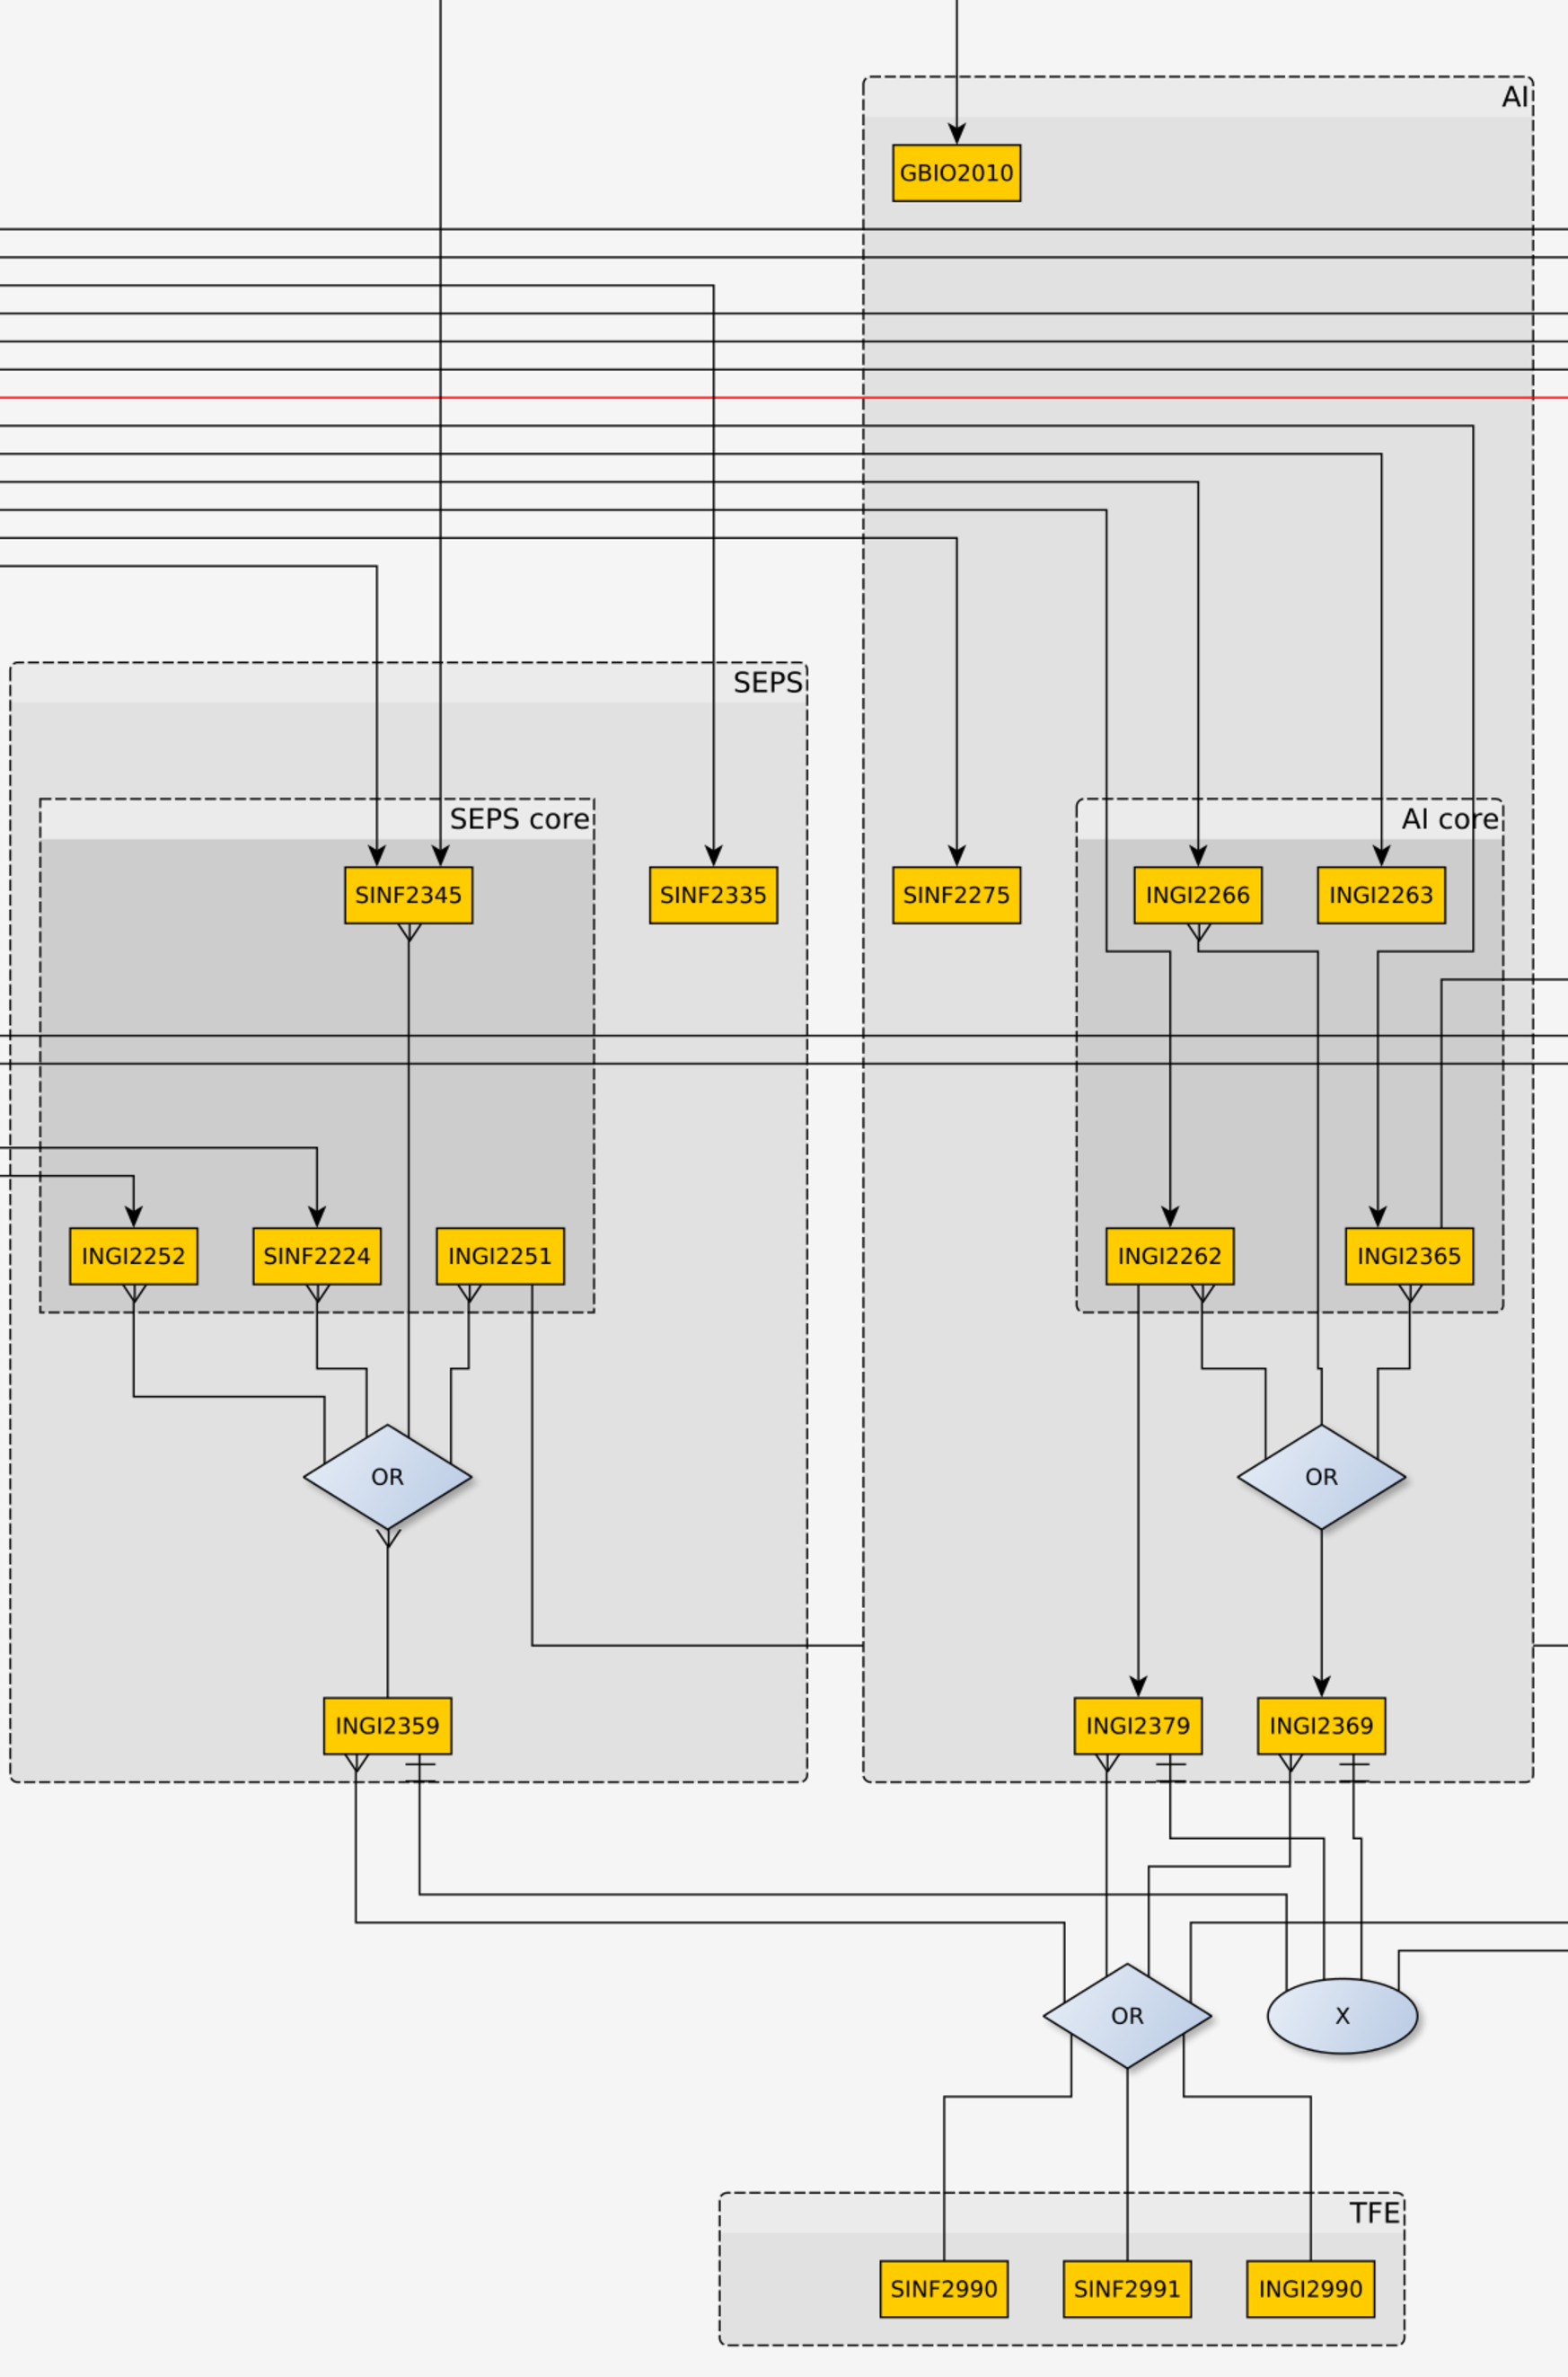
\includegraphics[width=0.8\textwidth]{ingi_sub_course_catalog}
\caption{Exemple de graph généré par Yed}
\label{fig:subcatalog}
\end{figure}

Les formats (non binaires) dans lesquels nous pouvons exporter les informations contenues dans notre graphe sont les suivantes. 
\begin{enumerate}
\item GraphML, un format de fichier basé sur XML pour les graphiques
\item XGML, une extensions du format GraphML
\item TGF (Trivial Graph Format) un format de fichier texte relativement simple pour décrire des graphiques
\end{enumerate}

TGF est de la forme

\begin{lstlisting}
1 SINF1101
2 FSAB1401
3 SINF1103
4 SINF1102
5 SINF1140
6 INGI1123
7 INGI1101
8 FSAB1402
9 NS //(Option network & security du programme Master)
\end{lstlisting}

et contient trop peu d'informations sur le graphe, comme les appartenances des cours aux différents modules et programmes. C'est pourquoi une solution basée sur XML a été choisie.

Voici ce à quoi ressemble les informations d'un fichier GraphML pour un noeud de type COURS.
\begin{lstlisting}
 <node id="n1::n3" yfiles.foldertype="group">
 	<data key="d5"/>
    <data key="d6">
    (...)
	<node id="n1::n3::n2">
  		<data key="d5"/>
  		<data key="d6">
    	  <y:ShapeNode>
      	  <y:Geometry height="30.0" width="68.0" x="1136.0" y="1541.453125"/>
      	  <y:Fill color="#FFCC00" transparent="false"/>
      	  <y:BorderStyle color="#000000" type="line" width="1.0"/>
      	  <y:NodeLabel alignment="center" autoSizePolicy="content" fontFamily="Dialog" fontSize="12" fontStyle="plain" hasBackgroundColor="false" hasLineColor="false" height="17.96875" modelName="internal" modelPosition="c" textColor="#000000" visible="true" width="61.57421875" x="3.212890625" y="6.015625">SINF2335</y:NodeLabel>
      	  <y:Shape type="rectangle"/>
    	  </y:ShapeNode>
 		 </data>
	</node>
	(...)
</node>
\end{lstlisting}

En comparaison, la version \textit{XGML} du même nœud.
\begin{lstlisting}
<section name="node">
	<attribute key="id" type="int">69</attribute>
	<attribute key="label" type="String">SINF2335</attribute>
	<section name="graphics">
		<attribute key="x" type="double">1170.0</attribute>
		<attribute key="y" type="double">1556.453125</attribute>
		<attribute key="w" type="double">68.0</attribute>
		<attribute key="h" type="double">30.0</attribute>
		<attribute key="type" type="String">rectangle</attribute>
		<attribute key="fill" type="String">#FFCC00</attribute>
		<attribute key="outline" type="String">#000000</attribute>
	</section>
	<section name="LabelGraphics">
		<attribute key="text" type="String">SINF2335</attribute>
		<attribute key="fontSize" type="int">12</attribute>
		<attribute key="fontName" type="String">Dialog</attribute>
		<attribute key="anchor" type="String">c</attribute>
	</section>
	<attribute key="gid" type="int">61</attribute>
</section>
\end{lstlisting}
\textcolor{red}{En préparant la liste des pour \& contre des deux formats, il apparaît clairement que le format graphml est mieux adapté au parsing .. si j'ai le temps je changerai vite fait le parseur, ça ne devrait pas prendre plus d'une après midi à coder. En attendant, je stop ici la justification du choix du format} 
\subsubsection{Construction et Import du formulaire Excel}
Comme expliqué précédemment, le graph à lui seul n'est pas suffisant pour ajouter toute les informations nécessaire à l'application. Le formulaire Excel est utilisé pour ajouter les informations relatives au propriétés des programmes, modules et cours des différents curricula. 

Ces propriétés contiennent des informations simples sur les différents objets du catalogues comme le nom complet des différents cours, modules et programmes, les professeurs, les liens vers pages des cours. Elle contiennent aussi les informations relatives aux contraintes sur les propriétés, comme le nombre de crédits.

Il n'y a aucune restrictions sur les informations qui peuvent être ajoutées ici. 

La structure du document est la suivante~\ref{fig:excel_structure}. Tout d'abord, il y a une page par objet (Cours, Programme, Module, Sous-module)

\begin{figure}[H]
\centering
\caption{Structure d'un formulaire Excel}
\label{fig:excel_structure}
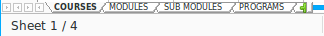
\includegraphics[width=0.8\textwidth]{excel_structure}
\end{figure}

Chacune des pages est structurée comme illustré sur l'image~\ref{fig:excel_page_structure}. 

\begin{figure}[H]
\centering
\caption{Structure de la page relatives aux cours du formulaire Excel}
\label{fig:excel_page_structure}
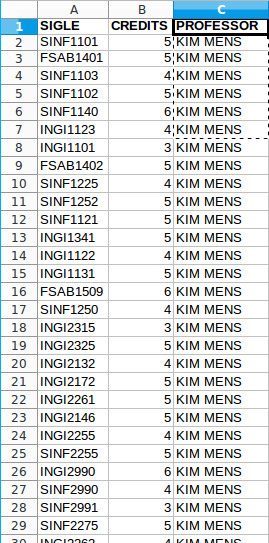
\includegraphics[scale=1]{excel_page_structure}
\end{figure}

La ligne 1, comprenant des cellules écrites en \textbf{gras} représente le header de la page. Chacune des cellules représente le nom de la propriété en question. Une propriété est un couple (Type, Value) où \textit{Type} correspond au nom de la propriété, et \textit{Value} à sa valeur. La première colomne représente la propriété qui \textbf{identifie} l'objet en question. Lorsque la page sera importé, une nouvelle propriété sera créée pour l'objet identifié par l'élément de la première colonne. La valeur de cette propriété sera la cellule traitée, et le type de la propriété le nom de la colonne. 

Par exemple, pour la ligne 4 de la page~\ref{fig:excel_page_structure}
Deux propriétés seront crées pour le cours intitulé \textit{SINF1103}
\begin{enumerate}
\item La propriété ayant pour type \textbf{CREDITS} avec comme valeur \textbf{5}.
\item La propriété ayant pour type \textbf{PROFESSOR} avec comme valeur \textbf{KIM MENS}.
\end{enumerate}

Pour plus de facilité, il est possible de télécharger un \textit{template} de se formulaire depuis l'application, contenant toute les informations qui existe dans la base de données. 

Par example, si l'on décide de télécharger ce template juste après avoir importer le graphe de cours, on aura les informations suivantes~\ref{fig:init_excel} pour les cours. 

\begin{figure}[H]
\caption{Formulaire excel téléchargé juste après importation du graphe}
\label{fig:init_excel}
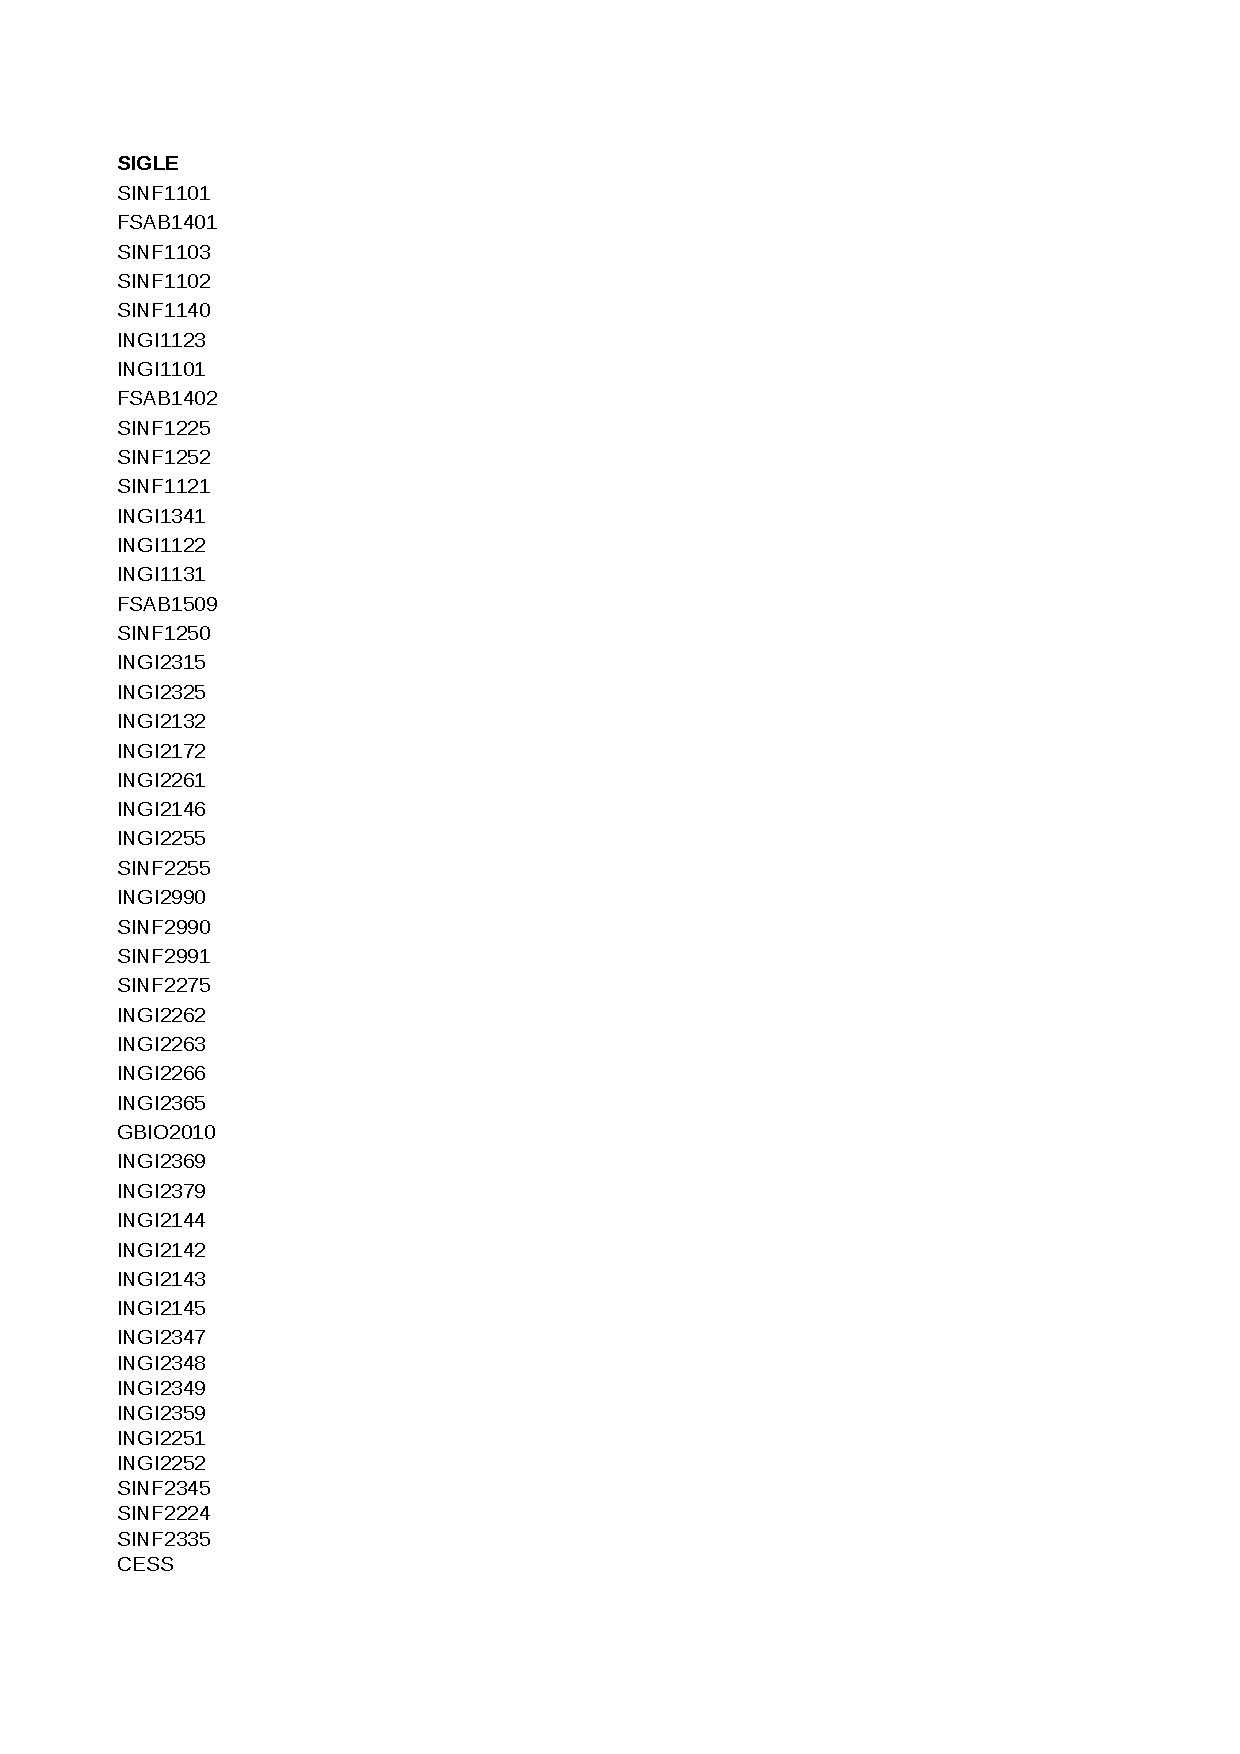
\includegraphics[scale=0.8]{init_excel}
\end{figure}

Il suffira après à la commission de programme de compléter ce fichier avec les informations souhaitées et de le télécharger vers l'application.

\clearpage
\section{Implémentation}
\subsection{Importation du graphe}
Le but de ce module est de fournir une abstraction supplémentaire à la gem "Nokogiri" pour parser le format xgml de yEd. Les informations contenue dans le graphe généré avec Yed sont les suivantes:
\begin{itemize}
\item Les Programmes de cours (Bachelier, Masters)
\item Les Modules et leur nom
\item Les Sous-modules et leur nom
\item Les cours et leur sigle
\item Les contraintes hiérarchiques (Qui contient quoi, qui dépend de qui.)
\end{itemize}

L'importation se fait via un fichier xml généré par Yed. XML signifie XML eXtensible Markup Language. Un document xml est composé d'élément hiérarchisés. Chaque élément peut avoir un enfant, est identifié par un tag, peut avoir des attributs et contient de l'information. Les deux éléments dont nous avons avons besoin sont les \textit{<section>} avec l'attribut
\begin{enumerate}
\item{\textbf{Node} : Ces éléments identifient les programmes, les modules, les sous-modules, les cours et les dépendances n-aires.
Les enfants contenant de l'information importante sont les suivants:\\
\begin{tabular}{ | c || c | c || c | }
\hline
\textbf{Attribut}: & \textbf{Nom} & \textbf{Type} & \textbf{Information}\\
\hline
\hline
& id & int & Identifiant de l'élément\\
\hline
& label & string & Nom de l'élément\\
\hline
& isGroup & boolean & Spécifie si l'élément est un groupe\\
\hline
& gid & int & Identifiant du groupe parent\\
\hline
& customconfiguration & boolean & Identifie les formes spéciales\\
\hline
\end{tabular}
}
\item
{
\textbf{Edge} : Ces éléments identifient les dépendances entre les cours. Ils se situent à la suite de tout les éléments \textit{"node"} dans le fichier xml (Nous allons voir par la suite pourquoi cela pause un problème dans le parsing).Les enfants contenant de l'information pertinente sont les suivants:\\
\begin{tabular}{ | c || c | c || c| }
\hline
\textbf{Attribut} & \textbf{Nom} & \textbf{Type} & \textbf{Information}\\
\hline
\hline
& source & int & Source de l'arrête\\
\hline
& target & int & Cible de l'arrête\\
\hline
& targetArrow & string & Type de l'arrête\\
\hline
\end{tabular}
}
\end{enumerate}

Le parsing est donc relativement simple. En utilisant la gem Nokogiri, on a aisément accès à toute les informations présentée plus haut. Cependant, on est obligé de parser le fichier xml de façon linéaire. En effet, yEd n'utilise pas à 100\% l'aspect hiérarchique du xml. Les nœuds sont stockés l'un a la suite de l'autre, alors qu'il pourrait être stockés en tant que fils de leur parents, s'il sont dans un groupe par exemple.

L'idée de l'algorithme de parsing est donc de parcourir chacun des éléments \textit{"node"} et dans extraire l'information nécessaire. \\
\begin{itemize}
\item Pour les nœuds, nous devons regarder les élément-enfant \textbf{label} et \textbf{id} pour les identifier. Pour identifier le type d'objet qu'il représente (Cours, Modules, ...), il faut aller regarder la valeur de l'élément \textbf{isGroup}. Ensuite, pour identifier le parent de l'objet, s'il y a, il faut aller recupérer la valeur contenue dans l'élément \textbf{gid}. Notons que pour les contraintes n-aire, il faut aller voir certains attributs spéciaux de l'élément (\textbf{cutomConfiguration} par example), car nous utilisons des formes spéciales pour les représenter.
\item Pour les arrêtes (edge), nous devons récupérer les identifiant contenu dans les éléments \textbf{source} et \textbf{target} pour identifier ses sommets. Enfin, il faut aussi aller regarder le contenu de l'élément \textbf{targetArrow}  pour identifier le type de la dépendance.
\end{itemize}
\subsection{Importation du formulaire Excel}
Le module est composé de deux parties: 
\begin{enumerate}
\item Un \textit{Reader} qui propose une fonction pour récupérer sous forme de tableau de hash les informations d'une page Excel, en lui fournissant \textbf{le nom de la page}, ainsi que \textbf{la propriété qui est utilisée pour identifier l'objet} (Le sigle pour les cours par exemple).
\item Un \textit{Writter} qui propose une fonction pour écrire des données dans une page d'un document Excel.
\end{enumerate}

L'intérêt de fournir une abstraction supplémentaire se situe sur la structure des documents échangés avec l'utilisateur. En effet, chaque document comporte plusieurs pages. Chacune d'entre elles contient des informations sur un des objets (Course, Sub-Module, Modules ou Program). Ces informations sont représentées par le Modèle \textit{Property} en base de données. Il est donc nécessaire d'avoir la première ligne de chacune de ces pages réservée pour y mettre le header afin de savoir pour chaque ligne à quel type de propriété l'information appartient.

Pour les cours par exemple, ce header est de la forme
\begin{tabular}{| c | c | c | c |}
\hline
\textbf{Sigle} & \textbf{Crédits} & \textbf{...} & \textbf{...}\\
\hline
\end{tabular}  
